

\subsection{The plain detector is non-trivial}

%%%%%%%%%%%%%%%%%%%%%%%%%%%%%%%%%%%%%%%%%%%%%%%%%%%%%%%%%%%%%%%%%%%%
% \begin{table}[ht]
% \centering
% {
% \tablestyle{5pt}{1.2}
% \begin{tabular}{lccc}
% \multicolumn{1}{l|}{plain-backbone detector} & AP$^\text{b}$ & \multicolumn{1}{c|}{$\text{AP}^\text{m}$} & FLOPs \\
% % \hshline
% % (dynamic)  & \cmark & \xmark & \cmark & \xmark & \cmark & \xmark & \cmark \\
% \shline
% \header{\textbf{Multi-scale detection head}} & \header{} & \header{} & \header{} \\
% \multicolumn{1}{l|}{ViTDet w/ Cascade \citep{li2022vitdet}} & 54.0 & \multicolumn{1}{c|}{46.7} & 1.1T \\
% \multicolumn{1}{l|}{BoxeR w/ SimpleFPN \citep{nguyen2022boxer}} & 55.4 & \multicolumn{1}{c|}{47.7} & 0.5T \\
% \hline
% \header{\textbf{Plain detection head}} & \header{} & \header{} & \header{}  \\
% \multicolumn{1}{l|}{\ours} & 55.4 & \multicolumn{1}{c|}{47.6} & 0.5T \\

% \end{tabular}
% }
% \vspace{0.1in}
% \caption{\textbf{Ablation on single-scale \vs multi-scale features in plain-backbone detection} on COCO \val set. We train BoxeR \citep{nguyen2022boxer} with SimpleFPN proposed in \citep{li2022vitdet} and report its performance. Compared to ViTDet as our baseline of plain-backbone detector, BoxeR w/ SimpleFPN outperforms the baseline. Surprisingly, \ours performs on par with BoxeR w/ SimpleFPN under the same FLOPs despite of using single-scale input.}
% \label{tab:compare}
% %\vspace{-0.34in}
% \end{table}


\begin{table}[t]
    \floatbox[\capbeside]{table}
    {\caption{\textbf{Single-scale \vs multi-scale feature map} on COCO object detection and instance segmentation using ViT-B as backbone. Compared to ViTDet, BoxeR performs better for both tasks with less FLOPs. Interestingly, \ours performs on par with BoxeR under the same FLOPs despite using only single-scale input ($\ddag$: BoxeR with SimpleFPN \citep{li2022vitdet}). \cs{What is benefit? Unclear from table.}}\label{tab:compare}}%
    {
    \footnotesize
    {
    \tablestyle{2pt}{1.2}
    \begin{tabular}{lccc}
    \multicolumn{1}{l|}{} & AP$^\text{b}\!\uparrow$ & \multicolumn{1}{c|}{$\text{AP}^\text{m}\!\uparrow$} & FLOPs$\downarrow$ \\
    % \hshline
    % (dynamic)  & \cmark & \xmark & \cmark & \xmark & \cmark & \xmark & \cmark \\
    \shline
    \rowcolor{yellow!50} \textbf{Multi-scale head} &  &  &  \\
    \multicolumn{1}{l|}{ViTDet \citep{li2022vitdet}} & 54.0 & \multicolumn{1}{c|}{46.7} & 1.1T \\
    \multicolumn{1}{l|}{BoxeR$^\ddag$ \citep{nguyen2022boxer}} & 55.4 & \multicolumn{1}{c|}{47.7} & 0.5T \\
    \hline
    \rowcolor{yellow!50} \textbf{Single-scale head} &  &  &   \\
    \multicolumn{1}{l|}{\ours} & 55.4 & \multicolumn{1}{c|}{47.6} & 0.5T \\
    \end{tabular}
    }
    }
\end{table}
    
    
%     %%%%%%%%%%%%%%%%%%%%%%%%%%%%%%%%%%%%%%%%%%%%%%%%%%%%%%%%%%%%%%%%%%%%
    
    
    %%%%%%%%%%%%%%%%%%%%%%%%%%%%%%%%%%%%%%%%%%%%%%%%%%%%%%%%%%%%%%%%%%%%
    \begin{table}[ht]
    \centering
    \footnotesize
    {
    {
    \subfloat[\label{tab:strat} \textbf{Strategy for scale-aware attention.}]
    {
    \tablestyle{6pt}{1.2}
    \begin{tabular}{l|cc}
    scale-aware strat. & AP$^\text{b}\!\uparrow$ & $\text{AP}^\text{m}\!\uparrow$ \\
    \shline
    base & 54.5 & 46.8 \\
    \hline
    i) fixed-scale & 55.0 & 47.2 \\
    \rowcolor{gray!25} ii) adaptive-scale & 55.4 & 47.6 \\
    %  & & \\
    \end{tabular}
    }
    
    \subfloat[\label{tab:feat_scale} \textbf{Scales of input feature map.}]
    {
    \tablestyle{7.5pt}{1.2}
    \begin{tabular}{l|cc}
    feature scale & AP$^\text{b}\!\uparrow$ & $\text{AP}^\text{m}\!\uparrow$ \\
    \shline
    base & 54.5 & 46.8 \\
    \hline
    1/4 & 55.4 & 47.7 \\
    \rowcolor{gray!25} 1/8 & 55.4 & 47.6 \\
    1/16 & 54.2 & 46.6 \\
    \end{tabular}
    }
    \subfloat[\label{tab:window_size} \textbf{Reference window size.}]
    {
    \tablestyle{7.5pt}{1.2}
    \begin{tabular}{l|cc}
    $s$ & AP$^\text{b}\!\uparrow$ & $\text{AP}^\text{m}\!\uparrow$ \\
    % \hshline
    % (dynamic)  & \cmark & \xmark & \cmark & \xmark & \cmark & \xmark & \cmark \\
    \shline
    base & 54.5 & 46.8 \\
    \hline
    16 & 55.1 & 47.4 \\
    \rowcolor{gray!25} 32 & 55.4 & 47.6 \\
    64 & 55.1 & 47.4 \\
    \end{tabular}
    }
    \subfloat[\label{tab:num_scale} \textbf{Number of window scales}.]
    {
    \tablestyle{7.5pt}{1.2}
    \begin{tabular}{l|cc}
    $n$ & AP$^\text{b}\!\uparrow$ & $\text{AP}^\text{m}\!\uparrow$ \\
    \shline
    base & 54.5 & 46.8 \\
    \hline
    2 & 54.6 & 47.0 \\
    \rowcolor{gray!25} 4 & 55.4 & 47.6 \\
    6 & 55.2 & 47.6 \\
    \end{tabular}
    }
    }
    }
    % \vspace{-0.7em}
    \caption{\label{tab:det_ablation} \textbf{Ablation on the design of attention mechanism} using a plain ViT backbone on COCO~\citep{lin2014mscoco} object detection and instance segmentation. \ours receives the single-scale input from ViT and makes predictions. Compared to the na\"ive baseline which employs BoxeR and box-attention \citep{nguyen2022boxer} with single-scale features, \ours improves performance of the plain detector.}
    \end{table}
    %%%%%%%%%%%%%%%%%%%%%%%%%%%%%%%%%%%%%%%%%%%%%%%%%%%%%%%%%%%%%%%%%%%%
    
    
%     \boldparagraph{Dataset, tasks \& evaluation.} In this study, we evaluate our method on COCO~\citep{lin2014mscoco}, a common detection and segmentation dataset, catering for object detection, instance segmentation, and panoptic segmentation tasks. The COCO dataset contains 118,000 training images and 5,000 validation images of 80 ``thing'' and 53 ``stuff'' categories. We report the average precision metric $\text{AP}^\text{b}$ for object detection and $\text{AP}^\text{m}$ for instance segmentation, and the panoptic quality metric $\text{PQ}$ for panoptic segmentation. In panoptic segmentation, the union of ``thing'' and ``stuff'' categories are considered whereas in object detection and instance segmentation, the ``thing'' categories are the main focus. We train our network on the \train split and evaluate on the \val split.
    
%     \boldparagraph{Implementation details.} By default, we use a single-scale feature map with adaptive-scale attention as described in \cref{sec:single_scale}. We initialize the backbone from MAE~\citep{he2022mae} pre-trained on ImageNet-1K without any labels. Unless otherwise specified, the hyper-parameters are the same as in \citep{nguyen2022boxer}. For all experiments, our optimizer is AdamW~\citep{loshchilov2019adamw} with a learning rate of 0.0001 and a weight decay of 0.05. The learning rate is linearly warmed up for the first 250 iterations and decayed at 0.9 and 0.95 fractions of the total number of training steps by a factor 10. ViT-B~\citep{dosovitskiy2021vit} is set as the backbone. The layer-wise learning rate decay of 0.7 and drop path rate of 0.3 is applied to the ViT backbone. The input image size is $1024\times1024$ with large-scale jitter \citep{shiasi2021lsjitter} between a scale range of $[0.1, 2.0]$. Due to the limit of our computational resources, we report the ablation study using the standard $5\times$ schedule setting \citep{shiasi2021lsjitter} with batch size of 16. Following \citep{li2022vitdet}, we also finetune our networks within 100 epochs and a batch size of 64 in the main experiments. As the main goal is to keep the architecture and training process simple, these settings are applied to all tasks (\ie, object detection, instance segmentation, and panoptic segmentation).
%     The code will be released.
    
    \subsection{Scale-aware attention mechanism improves detection on single-scale input}
    
    
    %%%%%%%%%%%%%%%%%%%%%%%%%%%%%%%%%%%%%%%%%%%%%%%%%%%%%%%%%%%%%%%%%%%%
    \begin{table}[t]
    \centering
    \footnotesize
    {
    {
    \subfloat[\label{tab:attn} {\bf Instance-attention \vs Masked instance-attention.} ]
    {
    \tablestyle{4pt}{1.2}
    \begin{tabular}{l|ccc}
    attention & PQ$\uparrow$ & PQ$^\text{Th}\!\uparrow$ & PQ$^\text{St}\!\uparrow$\\
    \shline
    instance-attention \citep{nguyen2022boxer} & 54.9 & 61.2 & 45.3 \\
    \rowcolor{gray!25} masked instance-attention & 55.3 & 61.6 & 45.8 \\
    \end{tabular}
    }
    \hspace{0.1in}%
    \subfloat[\label{tab:pdecoder} {\bf Number of high-resolution layers.}]
    {
    \tablestyle{8pt}{1.2}
    \begin{tabular}{l|ccc}
    $K$ & PQ$\uparrow$ & PQ$^\text{Th}\!\uparrow$ & PQ$^\text{St}\!\uparrow$\\
    \shline
    0 & 54.6 & 60.9 & 45.1 \\
    \rowcolor{gray!25} 1 & 55.3 & 61.6 & 45.8 \\
    \end{tabular}
    }
    }
    }
    % \vspace{-0.7em}
    \caption{\label{tab:pan_ablation} \textbf{Ablation on mask prediction adaptation} in a plain detector on COCO~\citep{lin2014mscoco} panoptic segmentation. The masked instance-attention along with high-resolution layers improve the performance of \ours on panoptic segmentation, showing its effectiveness in capturing fine-grained information.}
    \end{table}
    %%%%%%%%%%%%%%%%%%%%%%%%%%%%%%%%%%%%%%%%%%%%%%%%%%%%%%%%%%%%%%%%%%%%
    
    
    \boldparagraph{Ablation 1: A single-scale feature map is enough.} In \cref{tab:compare}, we first compare plain-backbone detectors with single-scale \vs multi-scale features. The baseline of our study is the ViTDet: which employs the plain ViT as the backbone and Cascade R-CNN \citep{cai2019cascadercnn} with \emph{multi-scale} feature maps from a simple feature pyramid (SimpleFPN) \citep{li2022vitdet} as its detection head. We also train BoxeR with the plain backbone ViT and SimpleFPN using a $5\times$ schedule for a better comparison.
    
    % Moreover, under the same amount of FLOPs, \ours with single-scale feature map performs on par with BoxeR with SimpleFPN. 
    From our observation, the single-scale feature map is sufficient and our adaptive-scale attention mechanism enables \ours to perform detection using plain features. As a result, \ours matches the performance of BoxeR under the same amount of FLOPs. This observation is different from BoxeR and recent end-to-end detection approaches \citep{zhu2021deformable,cheng2022mask2former} where a multi-scale feature map is needed to achieve competitive performance. We note that \ours follows a different perspective compared to convolution-based detection in \citep{chen2022uvit} when using a single-scale feature map. The convolution-based detection operates region-of-interest (RoI) pooling on object proposals to encode multi-scale information. Instead, our transformer-based encoder performs attention computation per feature vector to learn scale equivariant features. The significance of multiple feature maps diminishes when the encoder is equipped with a powerful attention mechanism.
    
    % It should be noted that different from the region proposal network (RPN) head in Mask R-CNN which performs region-of-interest (RoI) on the proposed regions of multiple scales, 
    
    
    %%%%%%%%%%%%%%%%%%%%%%%%%%%%%%%%%%%%%%%%%%%%%%%%%%%%%%%%%%%%%%%%%%%%
    \begin{figure}[!b]
    \centering
    
    \begin{minipage}{1\linewidth}
    \centering
    
    \begin{minipage}[b]{.24\linewidth}
    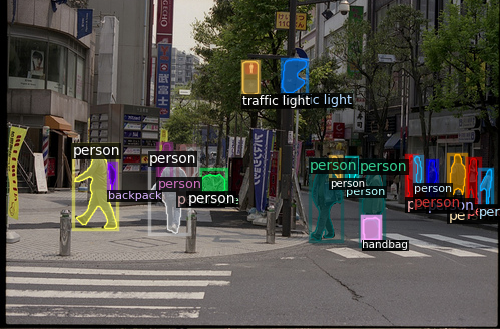
\includegraphics[width=\linewidth]{vis/success/val_848_det.png}
    \end{minipage}
    \begin{minipage}[b]{.24\linewidth}
    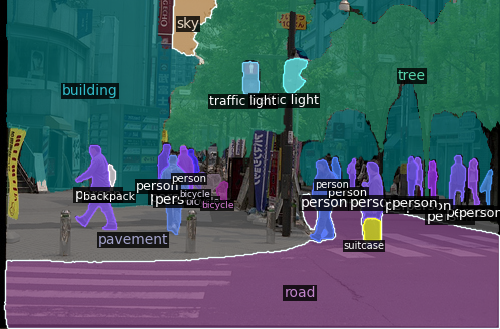
\includegraphics[width=\linewidth]{vis/success/val_848_pan.png}
    \end{minipage}
    \begin{minipage}[b]{.24\linewidth}
    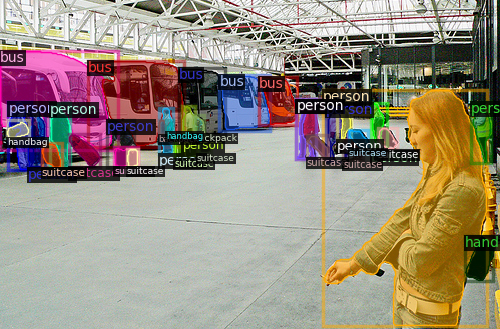
\includegraphics[width=\linewidth]{vis/success/val_965_det.png}
    \end{minipage}
    \begin{minipage}[b]{.24\linewidth}
    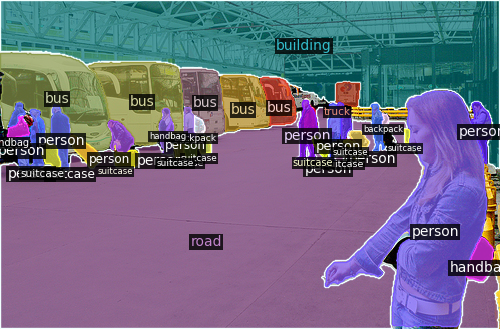
\includegraphics[width=\linewidth]{vis/success/val_965_pan.png}
    \end{minipage}
    
    \end{minipage}
    
    \caption{\textbf{Qualitative results} for object detection and panoptic segmentation on the COCO~\citep{lin2014mscoco} 2017 \val set generated by \ours. Note that \ours gives good predictions on small objects.}
    \label{fig:vis}
    % \vspace{-0.2in}
    \end{figure}
    %%%%%%%%%%%%%%%%%%%%%%%%%%%%%%%%%%%%%%%%%%%%%%%%%%%%%%%%%%%%%%%%%%%%
    
    \boldparagraph{Ablation 2: Scale-aware attention mechanism is an important factor.} \cref{tab:det_ablation} ablates the importance of the proposed attention mechanism. Here, we study the baseline which is the original box-attention from \citep{nguyen2022boxer} with a single-scale feature map of $\frac{1}{8}$ scale and window size of 32 pixels (denoted in ``base'') and the design choices of our scale-aware attention mechanism for detection.
    
    It can be seen from \cref{tab:strat} that both attention strategies of encoding multi-scale information in attention computation demonstrate strong detection performance. By allowing the feature vector to choose suitable scale information in its attended feature, our adaptive-scale attention obtains an improvement of 0.9 AP point over the baseline.
    
    In \cref{tab:feat_scale}, we verify the performance of \ours across multiple feature scales. The $\frac{1}{16}$ feature is created by applying a $1\times1$ convolution layer to the last ViT feature. For $\frac{1}{8}$ and $\frac{1}{4}$ feature, we use a transposed convolution layer. By default, we use \ours with adaptive-scale attention. Interestingly, the proposed method works well on $\frac{1}{16}$ features and performs worse than the baseline with $\frac{1}{8}$ features by a small gap of 0.3 AP point. The best trade-off between accuracy and efficiency comes from the features of $\frac{1}{8}$ scale. This results may align with DETR \citep{nicolas2020detr} where DETR-DC5 with dilated convolution in the C5 block shows better performance. In our case, we show that a simple transposed convolution layer is sufficient with plain ViT backbone.
    
    \cref{tab:window_size} compares the performance of \ours across several base sizes of the reference window. Our attention mechanism has only marginal differences in term of the base size. The ablation reveals that the number of scales in attention computation rather than the reference window size plays an important role to make our network scale-aware. Indeed, in \cref{tab:num_scale}, the use of multiple window scales shows improvement over the baseline. Increasing from 2 to 4 scales improves detection performance. This suggests that it is not trivial to be scale equivariant with a plain feature map and our adaptive-scale attention mechanism helps to strengthen features for detecting multi-scale objects.
    
    % To sum up, \cref{tab:det_ablation} shows that our proposed attention is an important factor for \ours to learn scale equivariant features in single-scale feature map. More importantly, it allows our network to operate on $\frac{1}{8}$ feature map which greatly reduces the computational requirement.
    
    \boldparagraph{Ablation 3: A single-scale architecture for panoptic segmentation.} We evaluate the effectiveness of our adaptations on panoptic segmentation in \cref{tab:pan_ablation}. The masked instance-attention outperforms the instance attention, an extension of box-attention for dense grid in \citep{nguyen2022boxer}, when keeping the same efficiency. Moreover, adding encoder layer on top of high-resolution feature map delivers a large gain in panoptic segmentation. This evidence confirms the capability of the encoder layer in learning both fine-grained and semantically meaningful features.
    
    \subsection{Main Results}
    
    %%%%%%%%%%%%%%%%%%%%%%%%%%%%%%%%%%%%%%%%%%%%%%%%%%%%%%%%%%%%%%%%%%%
    % \begin{table}[ht]
    % \centering
    % {
    % \tablestyle{2.8pt}{1.2}
    % \begin{tabular}{l|c|c|cccc|cccc|c}
    % \multirow{2}{*}{method} & plain & plain &  \multirow{2}{*}{AP$^\text{b}$} & \multirow{2}{*}{AP$^\text{b}_\text{S}$} & \multirow{2}{*}{AP$^\text{b}_\text{M}$} & \multirow{2}{*}{AP$^\text{b}_\text{L}$} & \multirow{2}{*}{$\text{AP}^\text{m}$} & \multirow{2}{*}{$\text{AP}^\text{m}_\text{S}$} & \multirow{2}{*}{$\text{AP}^\text{m}_\text{M}$} & \multirow{2}{*}{$\text{AP}^\text{m}_\text{L}$} &  \multirow{2}{*}{FLOPs} \\
    %  & backbone & head &  &  &  &  &  &  &  &  & \\
    % % \hshline
    % % (dynamic)  & \cmark & \xmark & \cmark & \xmark & \cmark & \xmark & \cmark \\
    % \shline
    % Swin$^\dag$ \citep{liu2021swintransformer} & \xmark & \xmark & 54.0 & - & - & - & 46.5 & - & - & - & 0.9T \\
    % MViT$^\dag$ \citep{fan2021mvit} & \xmark & \xmark & 55.6 & - & - & - & 48.1 & - & - & - & 0.8T \\
    % Mask2Former $(5\times)$ \citep{cheng2022mask2former} & \xmark & \xmark & - & - & - & - & 46.7 & 26.1 & 50.5 & 68.8 & 0.5T \\
    % \hline
    % UViT \citep{chen2022uvit} & \cmark & \cmark & 53.9 & - & - & - & 46.1 & - & - & - & 1.1T  \\
    % ViTDet \citep{li2022vitdet} & \cmark & \xmark & 54.0 & - & - & - & 46.7 & - & - & - & 1.1T \\
    % \ours $(5\times)$ & \cmark & \cmark & 55.4 & 36.1 & 59.1 & 70.9 & 47.6 & 26.8 & 51.4 & 67.1 & 0.5T \\
    % \ours & \cmark & \cmark & 55.6 & 37.1 & 59.2 & 71.6 & 48.0 & 27.5 & 51.5 & 67.8 & 0.5T \\
    % \end{tabular}
    % }
    % \vspace{0.1in}
    % \caption{\textbf{Comparison of plain \vs non-plain detectors in object detection} on the COCO 2017 \val set using the base backbone. By default, all backbones are pre-trained using ImageNet1K. \ours as a plain detector demonstrates competitive performance compared to many specialized models in instance detection and segmentation with a small amount of computation ($\dag$: backbones pre-trained on ImageNet-22K; $5\times$: methods fine-tuned using $5\times$ schedule). \cs{Should BoxeR be in this table? We could also add row with transformer backbone. Then it can be included in two categories. Plus it cannot do panoptic.}}
    % \label{tab:det_main}
    % % \vspace{-0.2in}
    % \end{table}
    
    
    \begin{table}[t!]
    \centering
    \footnotesize
    {
    {
    \tablestyle{2.5pt}{1.2}
    \begin{tabular}{lccccccccccccc}
    \multicolumn{1}{l|}{method} & \multicolumn{1}{c|}{backbone} &  AP$^\text{b}$ & AP$^\text{b}_\text{S}$ & AP$^\text{b}_\text{M}$ & \multicolumn{1}{c|}{AP$^\text{b}_\text{L}$} & $\text{AP}^\text{m}$ & $\text{AP}^\text{m}_\text{S}$ & $\text{AP}^\text{m}_\text{M}$ & \multicolumn{1}{c|}{$\text{AP}^\text{m}_\text{L}$} & PQ & PQ$^\text{Th}$ & \multicolumn{1}{c|}{PQ$^\text{St}$} & FLOPs \\
    % \hshline
    % (dynamic)  & \cmark & \xmark & \cmark & \xmark & \cmark & \xmark & \cmark \\
    \shline
    \rowcolor{yellow!50} \multicolumn{14}{l}{\footnotesize \textbf{Hierarchical, Multi-scale}} \\
    \multicolumn{1}{l|}{\textcolor{gray}{Swin$^\dag$} \citep{liu2021swintransformer}} & \multicolumn{1}{c|}{\textcolor{gray}{Swin-B}} & \textcolor{gray}{54.0} & \textcolor{gray}{-} & \textcolor{gray}{-} & \multicolumn{1}{c|}{\textcolor{gray}{-}} & \textcolor{gray}{46.5} & \textcolor{gray}{-} & \textcolor{gray}{-} & \multicolumn{1}{c|}{\textcolor{gray}{-}} & \multicolumn{3}{c|}{\small \textcolor{gray}{n/a}} & \textcolor{gray}{0.9T} \\
    \multicolumn{1}{l|}{\textcolor{gray}{MViT$^\dag$} \citep{fan2021mvit}} & \multicolumn{1}{c|}{\textcolor{gray}{MViT-B}} & \textcolor{gray}{55.6} & \textcolor{gray}{-} & \textcolor{gray}{-} & \multicolumn{1}{c|}{\textcolor{gray}{-}} & \textcolor{gray}{\textbf{48.1}} & \textcolor{gray}{-} & \textcolor{gray}{-} & \multicolumn{1}{c|}{\textcolor{gray}{-}} & \multicolumn{3}{c|}{\small \textcolor{gray}{n/a}} & \textcolor{gray}{0.8T} \\
    \multicolumn{1}{l|}{MaskFormer$(5\times)$ \citep{cheng2021maskformer}} & \multicolumn{1}{c|}{Swin-B} & \multicolumn{4}{c|}{\small n/a} & \multicolumn{4}{c|}{\small n/a} & 51.1 & 56.3 & \multicolumn{1}{c|}{43.2} & 0.4T \\
    \multicolumn{1}{l|}{Mask2Former$(5\times)$ \citep{cheng2022mask2former}} & \multicolumn{1}{c|}{Swin-B} & \multicolumn{4}{c|}{\small n/a} & 46.7 & 26.1 & 50.5 & \multicolumn{1}{c|}{\textbf{68.8}} & 55.1 & 61.0 & \multicolumn{1}{c|}{\textbf{46.1}} & 0.5T \\
    \hline
    \rowcolor{yellow!50} \multicolumn{14}{l}{\footnotesize \textbf{Plain, Multi-scale}} \\
    \multicolumn{1}{l|}{\textcolor{gray}{ViTDet} \citep{li2022vitdet}} & \multicolumn{1}{c|}{\textcolor{gray}{ViT-B}} & \textcolor{gray}{54.0} & \textcolor{gray}{-} & \textcolor{gray}{-} & \multicolumn{1}{c|}{\textcolor{gray}{-}} & \textcolor{gray}{46.7} & \textcolor{gray}{-} & \textcolor{gray}{-} & \multicolumn{1}{c|}{\textcolor{gray}{-}} & \multicolumn{3}{c|}{\small \textcolor{gray}{n/a}} & \textcolor{gray}{1.1T} \\
    \multicolumn{1}{l|}{BoxeR$^\ddag(5\times)$ \citep{nguyen2022boxer}} & \multicolumn{1}{c|}{ViT-B} & 55.4 & - & - & \multicolumn{1}{c|}{-} & 47.7 & - & - & \multicolumn{1}{c|}{-} & \multicolumn{3}{c|}{\small n/a} & 0.5T \\
    \hline
    \rowcolor{yellow!50} \multicolumn{14}{l}{\footnotesize \textbf{Simple, Plain}} \\
    \multicolumn{1}{l|}{\textcolor{gray}{UViT} \citep{chen2022uvit}} & \multicolumn{1}{c|}{\textcolor{gray}{UViT-B}} & \textcolor{gray}{53.9} & \textcolor{gray}{-} & \textcolor{gray}{-} & \multicolumn{1}{c|}{\textcolor{gray}{-}} & \textcolor{gray}{46.1} & \textcolor{gray}{-} & \textcolor{gray}{-} & \multicolumn{1}{c|}{\textcolor{gray}{-}} & \multicolumn{3}{c|}{\small \textcolor{gray}{n/a}} & \textcolor{gray}{1.1T}  \\
    \multicolumn{1}{l|}{\ours$(5\times)$} & \multicolumn{1}{c|}{ViT-B} & 55.4 & 36.1 & 59.1 & \multicolumn{1}{c|}{70.9} & 47.6 & 26.8 & 51.4 & \multicolumn{1}{c|}{67.1} & 55.3 & 61.6 & \multicolumn{1}{c|}{45.8} & 0.5T \\
    \multicolumn{1}{l|}{\ours} & \multicolumn{1}{c|}{ViT-B} & \textbf{55.6} & \textbf{37.1} & \textbf{59.2} & \multicolumn{1}{c|}{\textbf{71.6}} & 48.0 & \textbf{27.5} & \textbf{51.5} & \multicolumn{1}{c|}{67.8} & \textbf{55.6} & \textbf{62.1} & \multicolumn{1}{c|}{45.8} & 0.5T \\
    \end{tabular}
    }
    }
    % \vspace{-0.1in}
    \caption{\textbf{
    Universal detection and segmentation comparison} for object detection, instance segmentation, and panoptic segmentation on the COCO~\citep{lin2014mscoco} \val set. By default, all backbones are pre-trained using ImageNet1K. ($\dag$: backbones pre-trained on ImageNet-22K; $\ddag$: BoxeR with SimpleFPN from \citep{li2022vitdet}; $5\times$: methods fine-tuned using $5\times$ schedule; n/a: method is not applicable to the task). Methods in \textcolor{gray}{gray color} are with a convolution-based detection head. \ours as a plain detector demonstrates competitive performance compared to many specialized or end-to-end models with a small amount of computation and is the only one suited for all three tasks.}
    \label{tab:det_main}
    % \vspace{-0.2in}
    \end{table}
    %%%%%%%%%%%%%%%%%%%%%%%%%%%%%%%%%%%%%%%%%%%%%%%%%%%%%%%%%%%%%%%%%%%%
    
    \boldparagraph{Universal detection and segmentation.} \cref{tab:det_main} lists the performance of \ours \vs previous methods in object detection, instance segmentation and panoptic segmentation. 
    % The first part contains detectors with hierarchical backbone and multi-scale detection head while the second part shows the plain-backbone detectors using multi-scale features. The last row indicates plain detector with both plain backbone and single-scale head. 
    These approaches are divided into three parts: detectors with hierarchical backbone and multi-scale head, plain-backbone detectors using multi-scale features, and plain detector with both plain backbone and head.
    For plain-backbone methods, we report the performance of ViTDet \citep{li2022vitdet} and BoxeR w/ SimpleFPN \citep{nguyen2022boxer} fine-tuned on input image size of $1024\times1024$. Our method accounts for less FLOPs than convolution-based detection head. Across different detectors, \ours achieves strong performance on COCO object detection and instance segmentation. Interestingly, \ours outperforms Mask2Former \citep{cheng2022mask2former} in detecting small and medium objects but lags behind in large category. This makes \ours to be a competitive plain detector. In panoptic segmentation, we observe the same behaviour in which \ours improves over ``thing'' categories but lags behind in ``stuff'' categories. Overall, \ours, as a plain detector, can achieve highly accurate results on all three tasks and can compete with hierarchical and multi-scale detectors. Visualizations of \ours predictions are shown in \cref{fig:vis}.
    
    \boldparagraph{Limitations.} Our final goal is to simplify the detection pipeline and to achieve competitive results at the same time. In \cref{tab:compare} and \cref{tab:det_ablation}, we find that the attention mechanism which can effectively learn scale-aware information in its computation plays a key role for a plain detector. However, our adaptive-scale attention mechanism still encodes the knowledge of different scales. In the future, we hope that with the help of large-scale training data, a simpler design of the attention mechanism could also learn the scale equivariant property. Furthermore, \ours faces difficulties in detecting and segmenting large objects in the image. To overcome this limitation, we think that a design of attention computation which effectively combines both global and local information is necessary.
    % \mo{The first three sentences are not about limitations. Fig. \ref{fig:vis_2d} is not referenced in the text and with the current alignment looks like it is part of the limitations which is a bit unfortunate.}
    
    % %%%%%%%%%%%%%%%%%%%%%%%%%%%%%%%%%%%%%%%%%%%%%%%%%%%%%%%%%%%%%%%%%%%%
    % \begin{table}[ht]
    % \centering
    % {
    % \tablestyle{3pt}{1.2}
    % \begin{tabular}{l|c|c|ccc}
    % \multirow{2}{*}{method} & plain & plain & \multirow{2}{*}{PQ} & \multirow{2}{*}{PQ$^\text{Th}$} & \multirow{2}{*}{PQ$^\text{St}$} \\
    %  & backbone & head &  &  &    \\
    % % \hshline
    % % (dynamic)  & \cmark & \xmark & \cmark & \xmark & \cmark & \xmark & \cmark \\
    % \shline
    % MaskFormer \citep{cheng2021maskformer} & \xmark & \xmark & 51.1 & 56.3 & 43.2 \\
    % Mask2Former \citep{cheng2022mask2former} & \xmark & \xmark & 55.1 & 61.0 & 46.1 \\
    % \hline
    % \ours & \cmark & \cmark & 55.3 & 61.6 & 45.8 \\
    % % ours (ViT-B) & \cmark & \cmark & 55.6 & 61.8 & 46.2 \\
    % \end{tabular}
    % }
    % \vspace{0.1in}
    % \caption{\textbf{Comparison of plain \vs non-plain detectors in panoptic segmentation} on the COCO 2017 \val set using the base backbone. By default, backbones are pre-trained using ImageNet1K. All methods are fine-tuned using $5\times$ schedule. While lagging behind in segmenting ``stuff'' categories, \ours with single-scale feature input shows better overall performance, especially in ``thing'' categories.}
    % \label{tab:panoptic_main}
    % % \vspace{-0.2in}
    % \end{table}
    % %%%%%%%%%%%%%%%%%%%%%%%%%%%%%%%%%%%%%%%%%%%%%%%%%%%%%%%%%%%%%%%%%%%%
    
    
    
    % Moreover, we also demonstrate the effectiveness of our approach on long-tailed object detection and segmentation dataset, LVIS \citep{}. The LVIS dataset consists of 2M high-quality annotations of 1,203 classes with a natural, long-tailed distribution. The standard metrics are reported for LVIS dataset including $\text{AP}^\text{bbox}$ for object detection, $\text{AP}^\text{mask}$ for instance segmentation, $\text{AP}^\text{mask}_\text{rare}$ for instance segmentation of rare classes.
    
    % \boldparagraph{Implementation Details.}
    
    
    
    % \boldparagraph{Encoder.}
    
    
    
    % \boldparagraph{Object Decoder.}
    
    
    
    % \boldparagraph{Pixel Decoder.}
    
    
    % \boldparagraph{Prediction Head.}
    
    
    % \subsection{Ablation Studies}
    
    
    % \subsection{Main Results}
    
    

        

    %%%%%%%%%%%%%%%%%%%%%%%%%%%%%%%%%%%%%%%%%%%%%%%%%%%%%%%%%%%%%%%%%%%
    \begin{table}[h!]
        \centering
        \footnotesize
        {
        {
        \tablestyle{2.5pt}{1.2}
        \begin{tabular}{lcccccccccc}
        \multicolumn{1}{l|}{method} & \multicolumn{1}{c|}{backbone} &  AP$^\text{b}$ & AP$^\text{b}_\text{S}$ & AP$^\text{b}_\text{M}$ & \multicolumn{1}{c|}{AP$^\text{b}_\text{L}$} & $\text{AP}^\text{m}$ & $\text{AP}^\text{m}_\text{S}$ & $\text{AP}^\text{m}_\text{M}$ & \multicolumn{1}{c|}{$\text{AP}^\text{m}_\text{L}$} & FPS \\
        % \hshline
        % (dynamic)  & \cmark & \xmark & \cmark & \xmark & \cmark & \xmark & \cmark \\
        \shline
        \rowcolor{yellow!50} \multicolumn{11}{l}{\footnotesize \textbf{Hierarchical, Multi-scale}} \\
        \multicolumn{1}{l|}{\textcolor{gray}{Swin$^\dag$} \citep{liu2021swintransformer}} & \multicolumn{1}{c|}{\textcolor{gray}{Swin-B}} & \textcolor{gray}{54.0} & \textcolor{gray}{-} & \textcolor{gray}{-} & \multicolumn{1}{c|}{\textcolor{gray}{-}} & \textcolor{gray}{46.5} & \textcolor{gray}{-} & \textcolor{gray}{-} & \multicolumn{1}{c|}{\textcolor{gray}{-}} & 13 \\
        \multicolumn{1}{l|}{\textcolor{gray}{MViT$^\dag$} \citep{fan2021mvit}} & \multicolumn{1}{c|}{\textcolor{gray}{MViT-B}} & \textcolor{gray}{55.6} & \textcolor{gray}{-} & \textcolor{gray}{-} & \multicolumn{1}{c|}{\textcolor{gray}{-}} & \textcolor{gray}{\textbf{48.1}} & \textcolor{gray}{-} & \textcolor{gray}{-} & \multicolumn{1}{c|}{\textcolor{gray}{-}} & 11 \\
        \multicolumn{1}{l|}{Mask2Former$^\ddag$ \citep{cheng2022mask2former}} & \multicolumn{1}{c|}{Swin-B} & \multicolumn{4}{c|}{\small n/a} & 46.7 & 26.1 & 50.5 & \multicolumn{1}{c|}{\textbf{68.8}} & {\small n/a} \\
        % ************************************
        \multicolumn{1}{l|}{\textcolor{gray}{Swin$^\dag$} \citep{liu2021swintransformer}} & \multicolumn{1}{c|}{\textcolor{gray}{Swin-L}} & \textcolor{gray}{54.8} & \textcolor{gray}{-} & \textcolor{gray}{-} & \multicolumn{1}{c|}{\textcolor{gray}{-}} & \textcolor{gray}{47.3} & \textcolor{gray}{-} & \textcolor{gray}{-} & \multicolumn{1}{c|}{\textcolor{gray}{-}} & 10 \\
        \multicolumn{1}{l|}{\textcolor{gray}{MViT$^\dag$} \citep{fan2021mvit}} & \multicolumn{1}{c|}{\textcolor{gray}{MViT-L}} & \textcolor{gray}{55.6} & \textcolor{gray}{-} & \textcolor{gray}{-} & \multicolumn{1}{c|}{\textcolor{gray}{-}} & \textcolor{gray}{\textbf{48.1}} & \textcolor{gray}{-} & \textcolor{gray}{-} & \multicolumn{1}{c|}{\textcolor{gray}{-}} & 11 \\
        \multicolumn{1}{l|}{Mask2Former \citep{cheng2022mask2former}} & \multicolumn{1}{c|}{Swin-L} & \multicolumn{4}{c|}{\small n/a} & 46.7 & 26.1 & 50.5 & \multicolumn{1}{c|}{\textbf{68.8}} & {\small n/a} \\
        \shline
        \rowcolor{yellow!50} \multicolumn{11}{l}{\footnotesize \textbf{Plain, Multi-scale}} \\
        \multicolumn{1}{l|}{BoxeR$^\ddag$ \citep{nguyen2022boxer}} & \multicolumn{1}{c|}{ViT-B} & 55.4 & - & - & \multicolumn{1}{c|}{-} & 47.7 & - & - & \multicolumn{1}{c|}{-} & 12 \\
        \multicolumn{1}{l|}{\textcolor{gray}{ViTDet} \citep{li2022vitdet}} & \multicolumn{1}{c|}{\textcolor{gray}{ViT-B}} & \textcolor{gray}{54.0} & \textcolor{gray}{-} & \textcolor{gray}{-} & \multicolumn{1}{c|}{\textcolor{gray}{-}} & \textcolor{gray}{46.7} & \textcolor{gray}{-} & \textcolor{gray}{-} & \multicolumn{1}{c|}{\textcolor{gray}{-}} & 11 \\
        % ************************************
        \multicolumn{1}{l|}{\textcolor{gray}{ViTDet} \citep{li2022vitdet}} & \multicolumn{1}{c|}{\textcolor{gray}{ViT-L}} & \textcolor{gray}{54.0} & \textcolor{gray}{-} & \textcolor{gray}{-} & \multicolumn{1}{c|}{\textcolor{gray}{-}} & \textcolor{gray}{46.7} & \textcolor{gray}{-} & \textcolor{gray}{-} & \multicolumn{1}{c|}{\textcolor{gray}{-}} & 11 \\
        \shline
        \rowcolor{yellow!50} \multicolumn{11}{l}{\footnotesize \textbf{Simple, Plain}} \\
        \multicolumn{1}{l|}{\textcolor{gray}{UViT} \citep{chen2022uvit}} & \multicolumn{1}{c|}{\textcolor{gray}{UViT-B}} & \textcolor{gray}{53.9} & \textcolor{gray}{-} & \textcolor{gray}{-} & \multicolumn{1}{c|}{\textcolor{gray}{-}} & \textcolor{gray}{46.1} & \textcolor{gray}{-} & \textcolor{gray}{-} & \multicolumn{1}{c|}{\textcolor{gray}{-}} & 12 \\
        \multicolumn{1}{l|}{\ours$^\ddag$} & \multicolumn{1}{c|}{ViT-B} & 55.4 & 36.1 & 59.1 & \multicolumn{1}{c|}{70.9} & 47.6 & 26.8 & 51.4 & \multicolumn{1}{c|}{67.1} & 15 \\
        \multicolumn{1}{l|}{\ours} & \multicolumn{1}{c|}{ViT-B} & \textbf{55.6} & \textbf{37.1} & \textbf{59.2} & \multicolumn{1}{c|}{\textbf{71.6}} & 48.0 & \textbf{27.5} & \textbf{51.5} & \multicolumn{1}{c|}{67.8} & 15 \\
        % ************************************
        \multicolumn{1}{l|}{\ours} & \multicolumn{1}{c|}{ViT-L} & \textbf{55.6} & \textbf{37.1} & \textbf{59.2} & \multicolumn{1}{c|}{\textbf{71.6}} & 48.0 & \textbf{27.5} & \textbf{51.5} & \multicolumn{1}{c|}{67.8} & 15 \\
        \end{tabular}
        }
        }
        % \vspace{-0.1in}
        \caption{\textbf{Object detection and instance segmentation comparison} between methods using single-scale \vs feature pyramids on COCO~\citep{lin2014mscoco} \val set. By default, all backbones are pre-trained using ImageNet1K. Methods in \textcolor{gray}{gray color} are with the convolution-based detection head. ($\dag$: backbones pre-trained on ImageNet-22K; $\ddag$: methods trained with $5\times$ schedule; n/a: entry is not available).}
        \label{tab:det_main}
        % \vspace{-0.2in}
        \end{table}
        %%%%%%%%%%%%%%%%%%%%%%%%%%%%%%%%%%%%%%%%%%%%%%%%%%%%%%%%%%%%%%%%%%%%